\documentclass[12pt]{article}
\usepackage[utf8]{inputenc}

\usepackage{lmodern}

\usepackage{enumitem}
\usepackage[margin=2cm]{geometry}

\usepackage{amsmath, amsfonts, amssymb}
\usepackage{graphicx}
%\usepackage{subfigure}
\usepackage{tikz}
\usepackage{pgfplots}
\usepackage{multicol}

\usepackage{comment}
\usepackage{url}
\usepackage{calc}
\usepackage{subcaption}
\usepackage[indent=0pt]{parskip}
\usepackage{animate}

\usepackage{array}
\usepackage{blkarray,booktabs, bigstrut}
\usepackage{bigints}

\pgfplotsset{compat=1.16}

% MATH commands
\newcommand{\ga}{\left\langle}
\newcommand{\da}{\right\rangle}
\newcommand{\oa}{\left\lbrace}
\newcommand{\fa}{\right\rbrace}
\newcommand{\oc}{\left[}
\newcommand{\fc}{\right]}
\newcommand{\op}{\left(}
\newcommand{\fp}{\right)}

\newcommand{\bi}{\mathbf{i}}
\newcommand{\bj}{\mathbf{j}}
\newcommand{\bk}{\mathbf{k}}
\newcommand{\bF}{\mathbf{F}}

\newcommand{\mR}{\mathbb{R}}

\newcommand{\ra}{\rightarrow}
\newcommand{\Ra}{\Rightarrow}

\newcommand{\sech}{\mathrm{sech}\,}
\newcommand{\csch}{\mathrm{csch}\,}
\newcommand{\curl}{\mathrm{curl}\,}
\newcommand{\dive}{\mathrm{div}\,}

\newcommand{\ve}{\varepsilon}
\newcommand{\spc}{\vspace*{0.5cm}}

\DeclareMathOperator{\Ran}{Ran}
\DeclareMathOperator{\Dom}{Dom}

\newcommand{\exo}[1]{\noindent\textcolor{red}{\fbox{\textbf{Problem {#1}}}\hrulefill}\\}
\newcommand{\qu}[4]{\noindent\textcolor{#4}{\fbox{\textbf{Section {#1} | Problem {#2}}} \hrulefill{{\fbox{\textbf{{#3} Points}}}}\\}}

\newcommand{\semester}{Spring 2023}

\newcommand{\CVup}{%

\begin{tikzpicture}
\draw[black, <->, >=latex] (-0.33, 0.5) .. controls (-0.125, 0) and (0.125, 0) .. (0.33, 0.5);
\end{tikzpicture}}

\newcommand{\CVupInc}{%
\begin{tikzpicture}
\draw[black, ->, >=latex] (0,0) .. controls (0.2, 0) and (0.4, 0.2) .. (0.5, 0.5);
\end{tikzpicture}}

\newcommand{\CVupDec}{%
\begin{tikzpicture}[rotate=270]
\draw[black, ->, >=latex] (0,0) .. controls (0.2, 0) and (0.4, 0.2) .. (0.5, 0.5);
\end{tikzpicture}}

\newcommand{\CVdown}{%
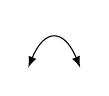
\begin{tikzpicture}
\draw[black, <->, >=latex] (-0.33, -0.5) .. controls (-0.125, 0) and (0.125, 0) .. (0.33, -0.5);
\end{tikzpicture}}

\newcommand{\CVdownInc}{%
\begin{tikzpicture}
\draw[black, ->, >=latex] (-0.5, -0.5) .. controls (-0.5, -0.3) and (-0.5, -0.1) .. (0,0);
\end{tikzpicture}}

\newcommand{\CVdownDec}{%
\begin{tikzpicture}[rotate=-90]
\draw[black, ->, >=latex] (-0.5, -0.5) .. controls (-0.5, -0.3) and (-0.5, -0.1) .. (0,0);
\end{tikzpicture}}

\begin{document}
	\noindent \hrulefill \\
	MATH-241 \hfill Pierre-Olivier Paris{\'e}\\
	Solutions Section 5-1 \hfill \semester \\\vspace*{-1cm}
	
	\noindent\hrulefill
	
	\spc	
	
	\exo{8}
	\\
	The intersections between $x^2 - 4x$ and $2x$ is given by the solutions to
		\begin{align*}
		x^2 - 4x = 2x \iff x^2 - 6x = 0 \iff x = 6 \text{ or } x = 0 .
		\end{align*}
	To have
		\begin{align*}
		x^2 - 4x \leq 6x \iff x (x - 6) \leq 0
		\end{align*}
	the value of $x$ should be between $0$ and $6$ ($0 \leq x \leq 6$). Therefore, the region is enclosed by the curve $6x$ (top/ceiling) and $x^2 - 4x$ (bottom/floor) from $x = 0$ to $x = 6$.
		\begin{center}
		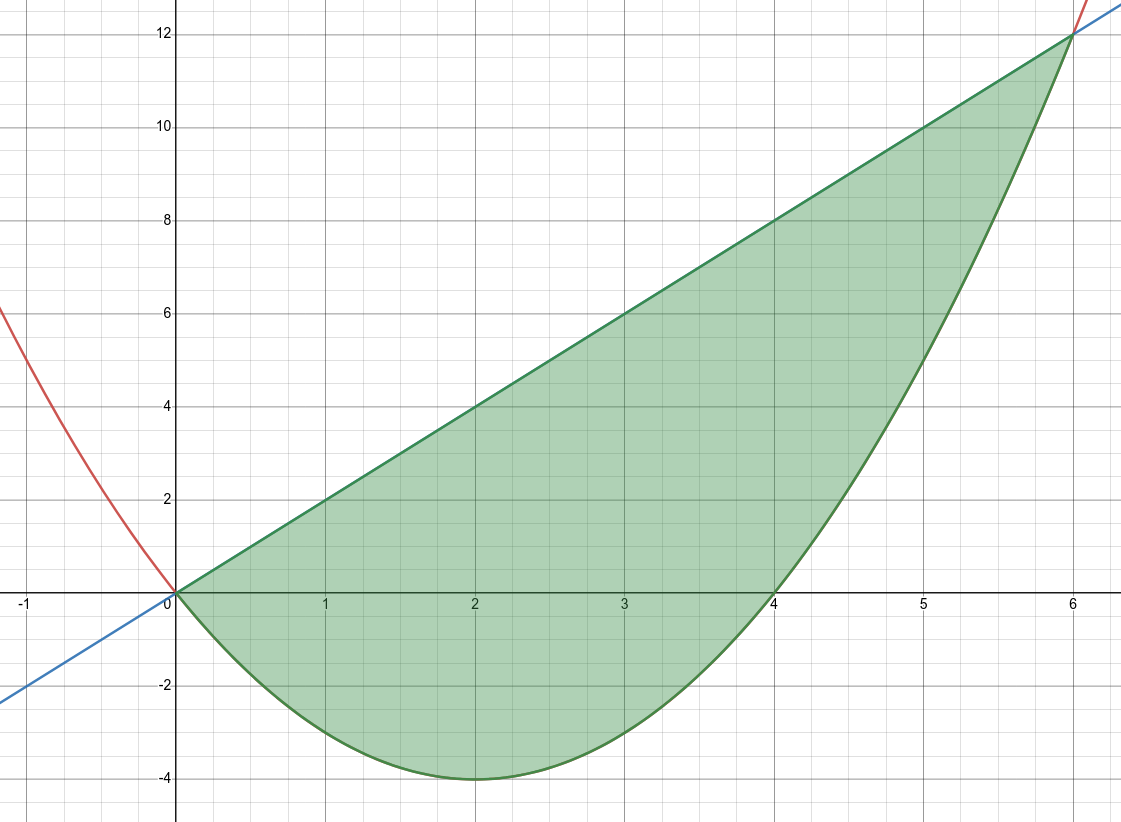
\includegraphics[scale=0.3]{fig1.png}
		\end{center}
		
	Therefore, the area of the region is given by
		\begin{align*}
		\int_0^6 2x - (x^2 - 4x) \, dx = \int_0^6 6x - x^2 \, dx = \left. \big( 3x^2 - \frac{x^3}{3} \big)\right|_0^6 = 36.
		\end{align*}
		
	\newpage
	
	\exo{12}
	\\
	The sketch of the region is the following:
		\begin{figure}[h]
		\centering
		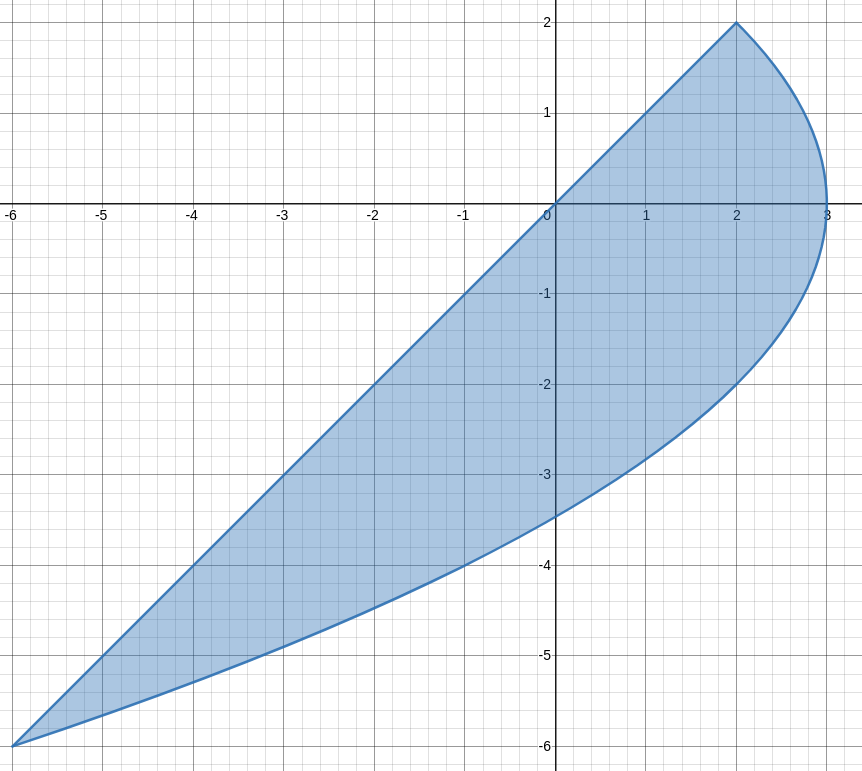
\includegraphics[scale=0.3]{exo-12}
		\end{figure}
		
	The intersections between the two curves are
		\begin{align*}
		4y + y^2 = 12 \iff y^2 + 4y - 12 = 0 \iff y = -6 \text{ or } y = 2 .
		\end{align*}
		
	We now have
		\begin{align*}
		A(S) = \int_{-6}^2 x_R - x_L \, dy = \int_{-6}^2 3 - y^2/4 - y \, dy = 64/3 .
		\end{align*}
		
	\newpage
	
	\exo{14}
	\\
	The sketch of the region:
		\begin{figure}[h]
		\centering
		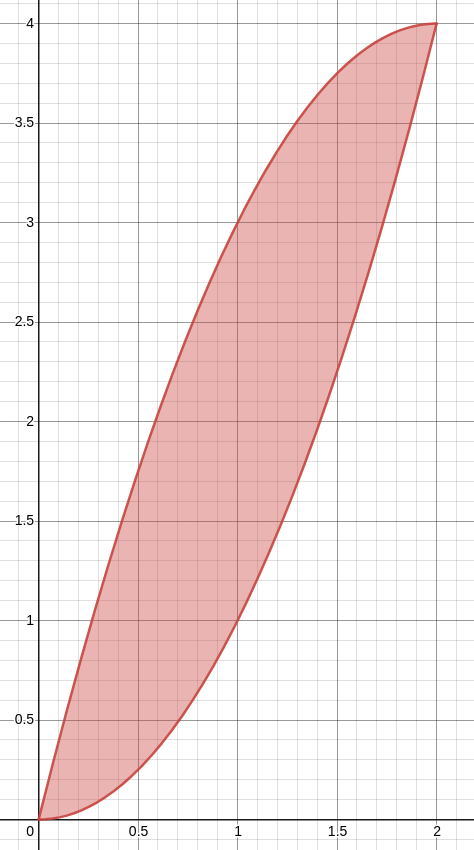
\includegraphics[scale=0.3]{exo-14}
		\end{figure}
		
	The intersections between the two curves are
		\begin{align*}
		x^2 = 4x - x^2 \iff x^2 - 2x = 0 \iff x = 0 \text{ or } x = 2 .
		\end{align*}
	So, we have
		\begin{align*}
		A (S) = \int_0^2 (4x - x^2) - (x^2) \, dx = 8/3 .
		\end{align*}
	
	\newpage
	
	\exo{18}
	\\
	The second curve is $y = x - 1$. The intersections between the two curves are
		\begin{align*}
		\sqrt{x - 1} = x - 1 \iff x - 1 = (x - 1)^2 \iff (x-2)(x-1) = 0
		\end{align*}
	and therefore $x = 1$ or $x = 2$. Here is the region between the two curves.
		\begin{center}
		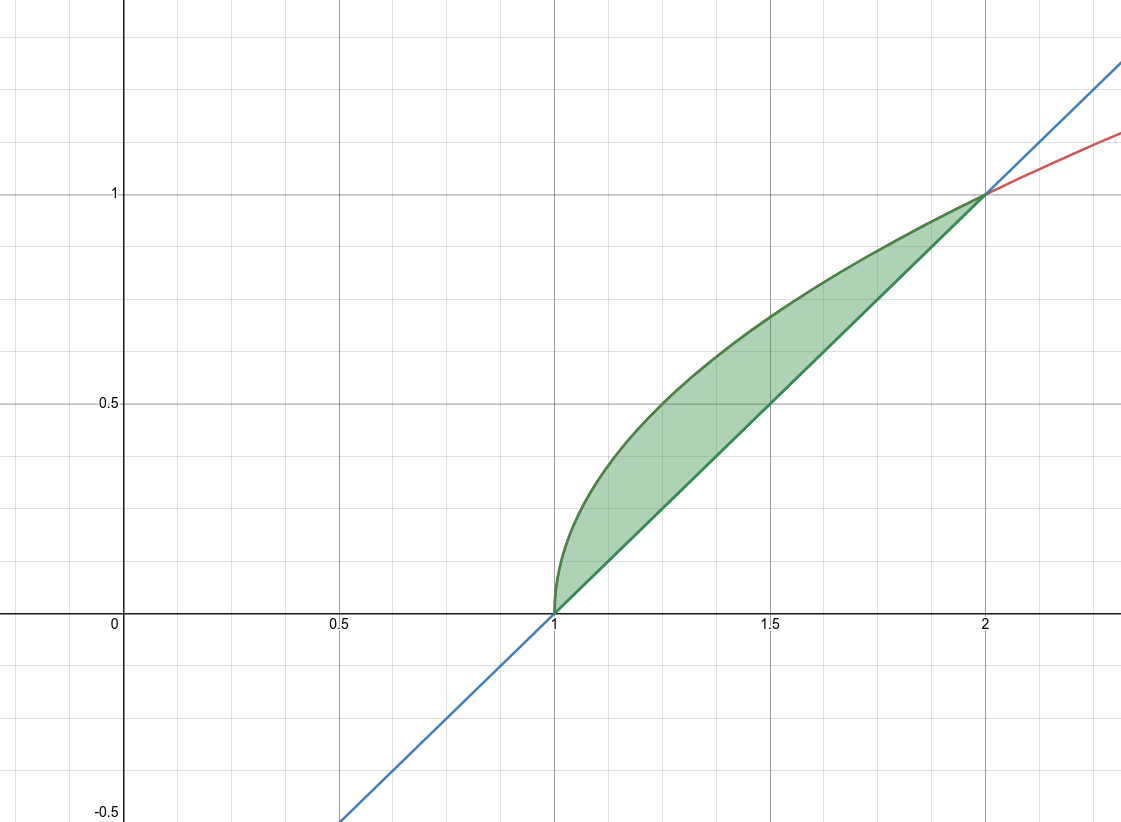
\includegraphics[scale=0.3]{fig2.png}
		\end{center}
		
	We have $\sqrt{x - 1} \geq x - 1$ for $1 \leq x \leq 2$. The area of the region is therefore
		\begin{align*}
		\int_1^2 \sqrt{x - 1} - (x - 1) \, dx = \int_1^2 \sqrt{x-1} \, dx - \int_1^2 x - 1 \, dx
		\end{align*}
	For the first integral, use a change of variable. Set $u = x - 1$, then $du = dx$ and
		\begin{align*}
		\int_1^2 \sqrt{x-1} \, dx = \int_0^1 \sqrt{u} \, du = \left. \big( \frac{2}{3} u^{3/2} \big)\right|_0^1 = \frac{2}{3} .
		\end{align*}
	Also, we have
		\begin{align*}
		\int_1^2 (x - 1) \, dx = \left. \big( \frac{x^2}{2} - x \big) \right|_1^2 = (2 - 2) - (1/2 - 1) = 1/2 .
		\end{align*}
	Therefore, the area is
		\begin{align*}
		\int_1^2 \sqrt{x - 1} - (x - 1) \, dx = \frac{2}{3} - \frac{1}{2} = \frac{1}{6} .
		\end{align*}
	
	
\end{document}